Este capítulo apresentará o método proposto por este trabalho para o projeto de uma prótese ativa baseada em sensores e aprendizado de máquina.

\section{Visão geral do método}
\label{sec:metodo_protese}

O projeto desenvolvido neste trabalho é uma prótese robótica para membros inferiores ou, mais especificamente, para a articulação do tornozelo. Esta prótese será construída a partir de modelos de próteses para impressoras 3D, aproveitando-se as partes mecânicas. A intenção é manter um baixo custo de produção. O sistema é projetado para funcionar em uma prótese transtibial, atuando sobre ela para adaptar a rigidez da articulação conforme a situação.

\begin{figure}[h]
	\caption{\label{fig:big_picture}Visão geral do protótipo}
	\begin{center}
	    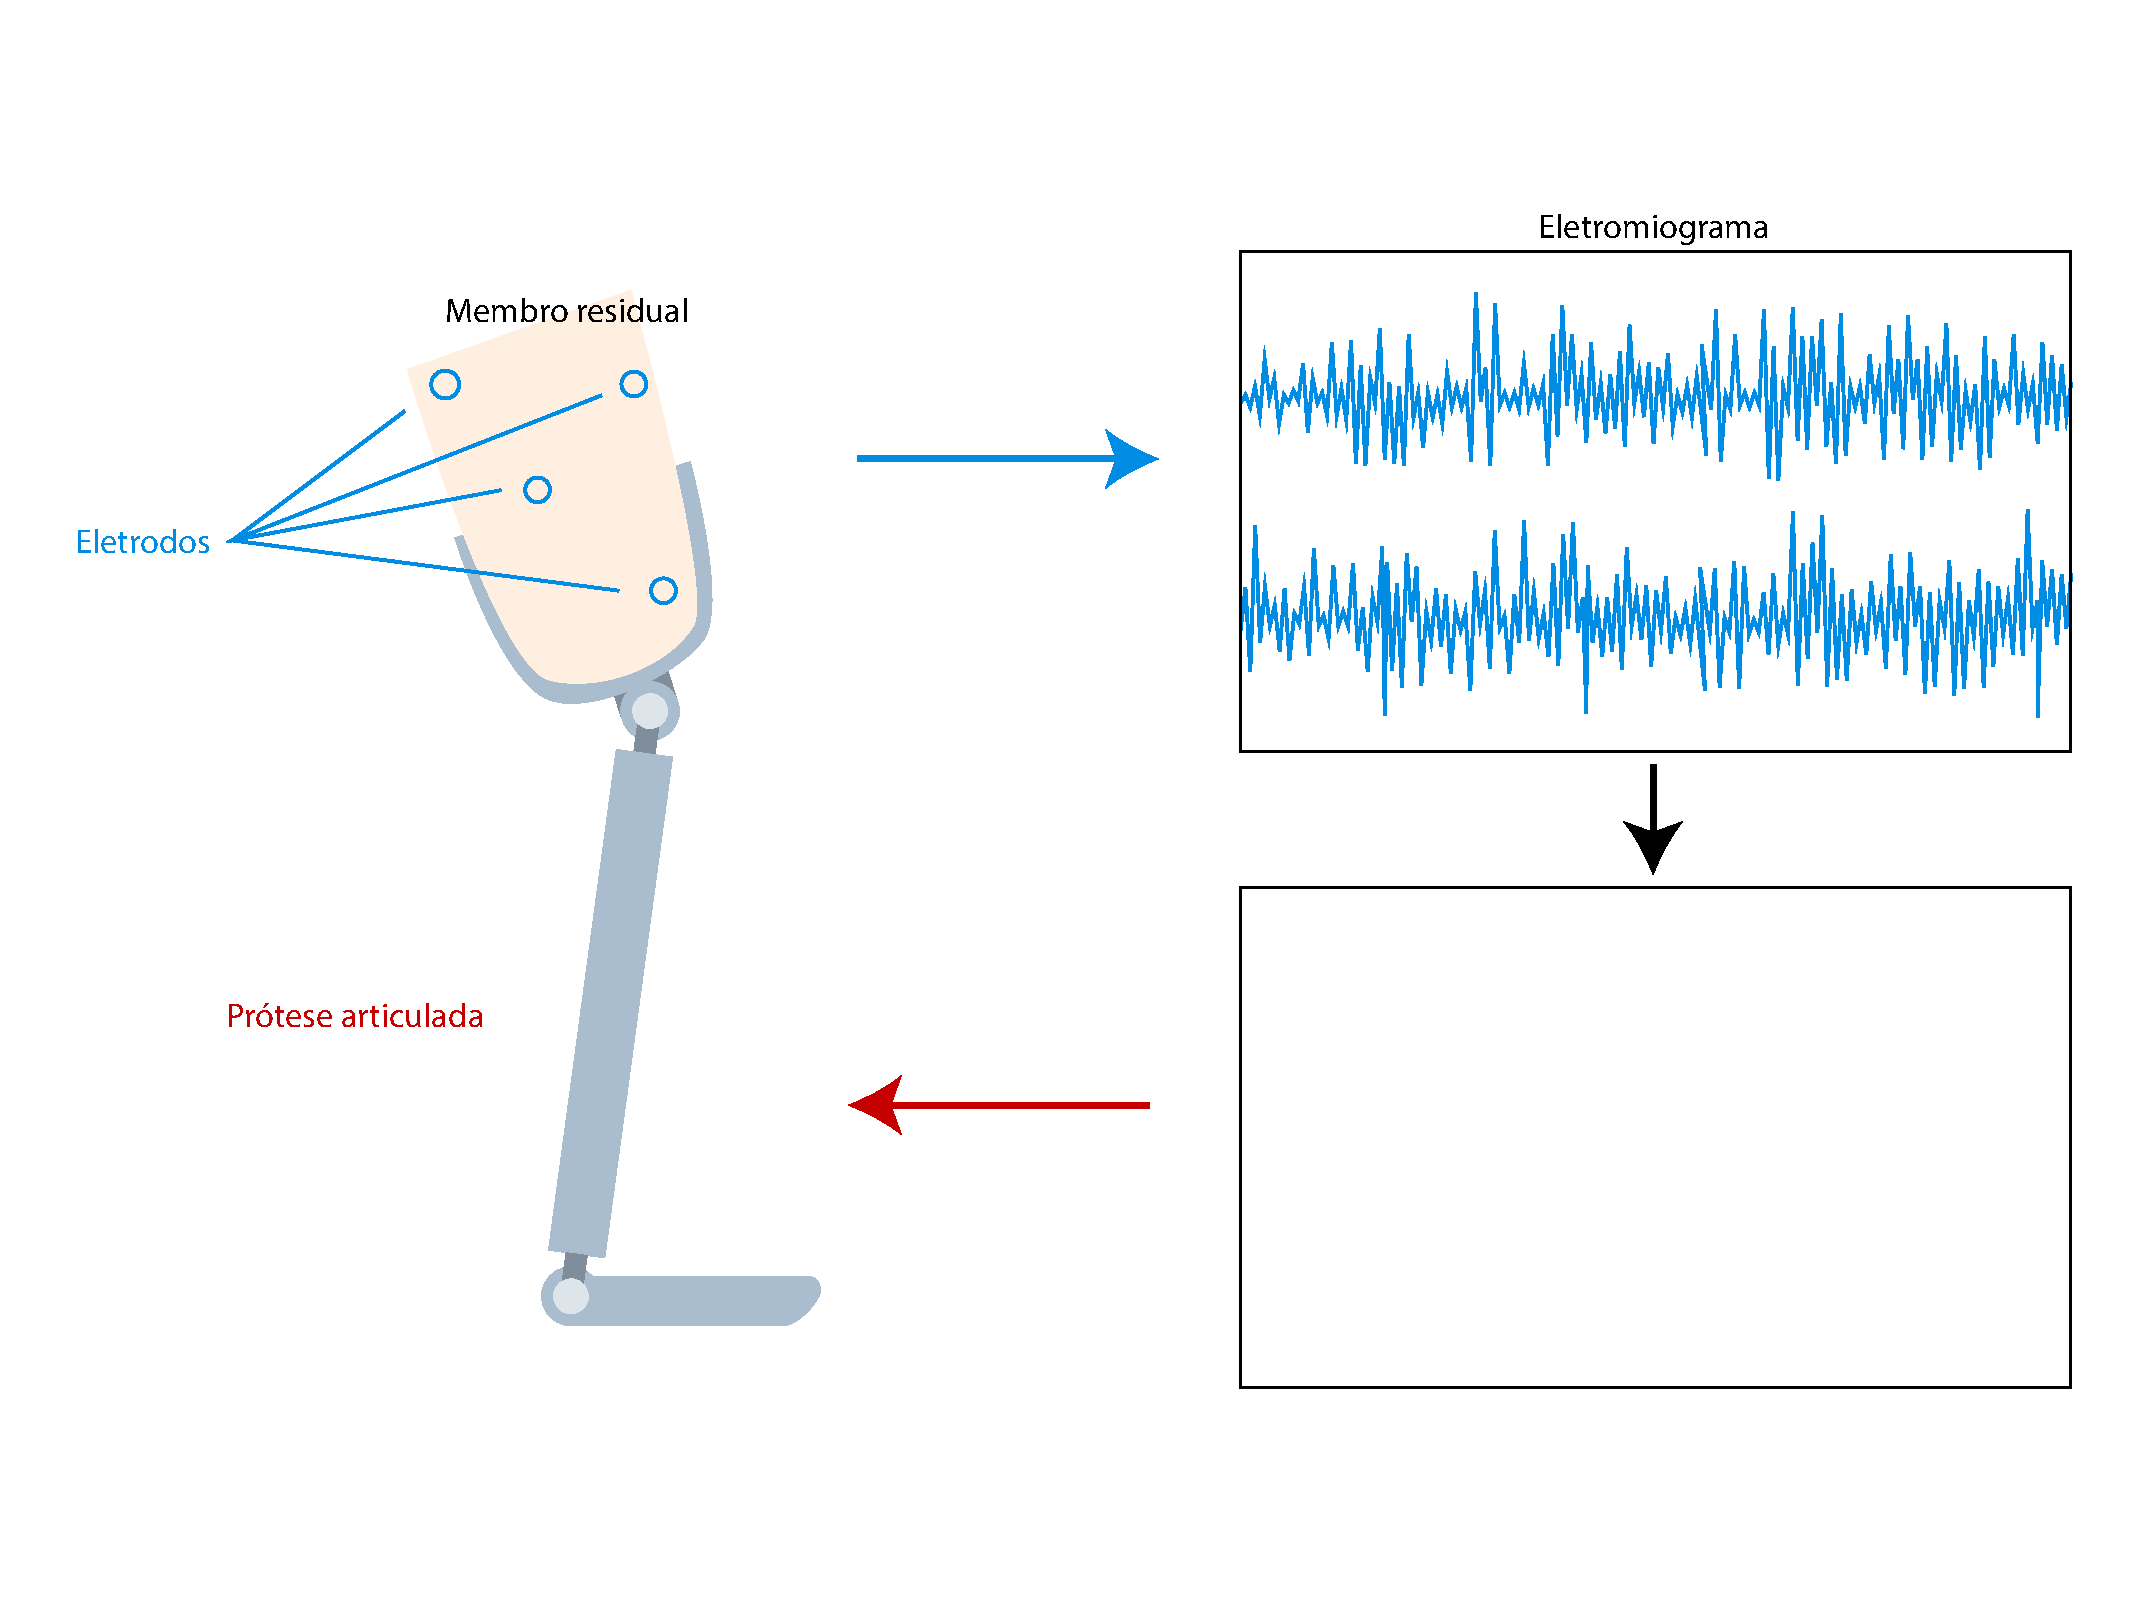
\includegraphics[width=0.6\textwidth]{resources/big_picture}
	\end{center}
	\legend{Fonte: Elaborada pelo autor}
\end{figure}

O sistema computacional que envolve o projeto estará equipado com sensores flex nas articulações dos joelhos além de giroscópios e acelerômetros, que serão usados para capturar as ações do usuário. A figura~\ref{fig:big_picture} ilustra a visão geral do sistema, incluindo o posicionamento dos sensores e o atuador da prótese em si.

Os sensores serão posicionados nos joelhos do usuário, e os dados capturados serão transmitidos a uma placa de processamento, que se comunicará com o atuador, de forma a adaptar a pisada do usuário de acordo com o ambiente. Conforme mostra a figura~\ref{fig:flowchart}, a prótese terá diferentes ajustes dependendo do tipo de ação, seja em caminhadas em planos, subida ou descida de escadas.

\todo{Terminar o fluxograma}\begin{figure}[h]
	\caption{\label{fig:flowchart}Fluxograma de funcionamento da prótese}
	\begin{center}
	    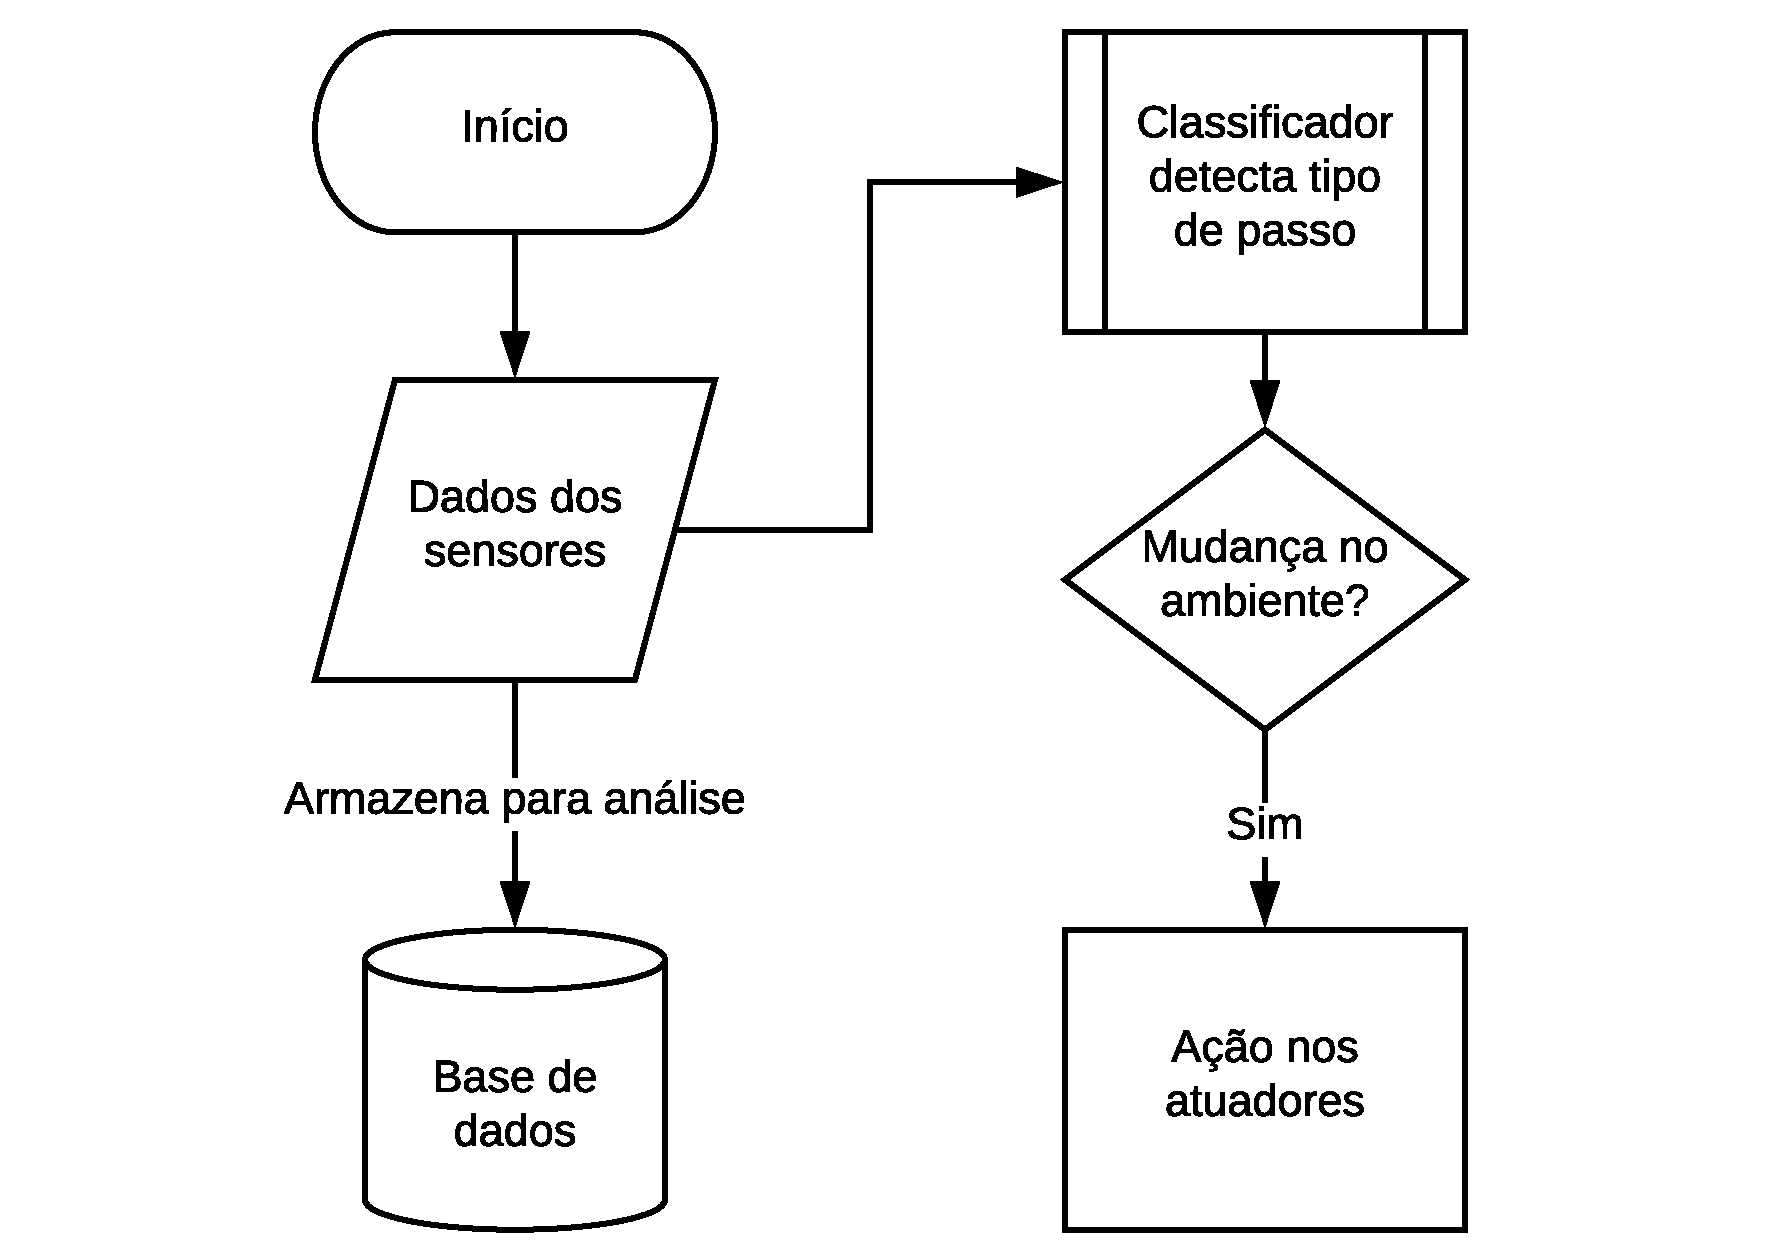
\includegraphics[width=\textwidth]{resources/flowchart}
	\end{center}
	\legend{Fonte: Elaborada pelo autor}
\end{figure}

\section{Prototipação da prótese}
\todo[inline,color=lightgray]{Descrever o funcionamento da prótese via algum modelo}
\subsection{Arquitetura do software}
\todo[inline,color=lightgray]{Diagrama UML}
\subsection{Arquitetura do hardware}
\todo[inline,color=lightgray]{Descrever os componentes da prótese: o motor, como funciona o motor e tal}

\section{Coleta de dados}
\todo[inline,color=lightgray]{Descrever que dados serão coletados (de que sensores) e como serão coletados, armazenados, etc.}

\section{Previsão de movimentos}
\todo[inline,color=lightgray]{Como, a partir da perna inteira, e do membro residual, identificar os movimentos para as ações necessárias. Descrever os cenários.
Identificar o tipo de ML: supervisionada, etc. Exemplos de algoritmos a serem utilizados baseados nos cenários.}
\todo[inline,color=lightgray]{Geração de movimentos: a partir dos dados coletados. Os atuadores vão tentar identificar os ambientes. Na escada, o motor vai fazer tal coisa, etc. Na rampa, etc.}


\section{Diagnóstico do uso da prótese e recomendações de melhorias no caminhar}
\todo[inline,color=lightgray]{Descrever a partir de que dados será feito o diagnóstico, bem como as recomendações. Os dados serão comparados com algum guideline de ortopedia.
(investigar para TCC2 se os sensores escolhidos são capazes de validar)}
\todo[inline,color=lightgray]{Analisar saúde do caminhar. Se não tá caminhando torto. Gerar estatísticas do uso da prótese. (Os dados estão fazendo a pessoa puxar mais pra uma perna)}
